\section{Results}
\label{sec:results}
In this section, we discuss our findings and threats to their validity.

\subsection{RQ: To  what  degree  do  the  results  of  extraction  share similarity with the actual extraction spit by experts?}

We assessed the similarity of the results from selected techniques and the ground-truths using MoJoFM as described in Section~\ref{sec:metric}. Table
\ref{tab:mojo-results} provides the MoJoFM results of the three architectures against which we assessed the selected extraction techniques.

\begin{table*}
\centering
\caption{MoJoFM results}
\label{tab:mojo-results}
\begin{tabular}{@{}|l|c|c|c|c|c|@{}}
\toprule
                  & \multicolumn{1}{l|}{Ground truth}       & \multicolumn{2}{c|}{Bunch}                                                       & \multicolumn{2}{c|}{FoSCI}                                                       \\ \midrule
Benchmark         & \multicolumn{1}{l|}{Number of services} & \multicolumn{1}{l|}{Number of services} & \multicolumn{1}{l|}{MoJoFM Similarity} & \multicolumn{1}{l|}{Number of services} & \multicolumn{1}{l|}{MoJoFM Similarity} \\ \midrule
JPetstore         & 3                                       & 3                                       & 66.67\%                                & 3                                       & 66.67\%                                \\ \midrule
Everest           & 4                                       & 4                                       & 25.00\%                                & 4                                       & 22.22\%                                \\ \midrule
PartsUnlimitedMRP & 5                                       & 7                                       & 81.98\%                                & 5                                       & 92.86\%                                \\ \bottomrule
\end{tabular}
\end{table*}

For all the three benchmarks, Neither \bn nor \fs performs significantly better than the other. For JPetstore, the two techniques produce the same level similarity, and \bn has a slightly higher similarity value than \fs does in Everest, while \fs does a better splitting in PartsUnlimitedMRP.

Due to the non-deterministic property of \bn, the clustering results vary between different runs. To illustrate the significant differences between runs, we perform a total of twenty times experiments using \bn under the same default parameters against the PartsUnlimitedMRP benchmark, and the result is shown in the figure \ref{fig:mq-vs-num-of-cluster-plot}. We plot the MQ value of the result for each run against the number of clusters. We intend to ignore the detail information, such as the internal differences of each cluster between multiple runs. If the individual differences are taken into consideration, the differences between runs would be even more substantial. The MQ values vary from 1.7 to 33.9, and the number of clusters varies from 3 to 10. For runs that have the same number of clusters, the MQ values are not in a reasonable small range, indicating the internal differences between each cluster are very huge.

\begin{figure}
    \centering
    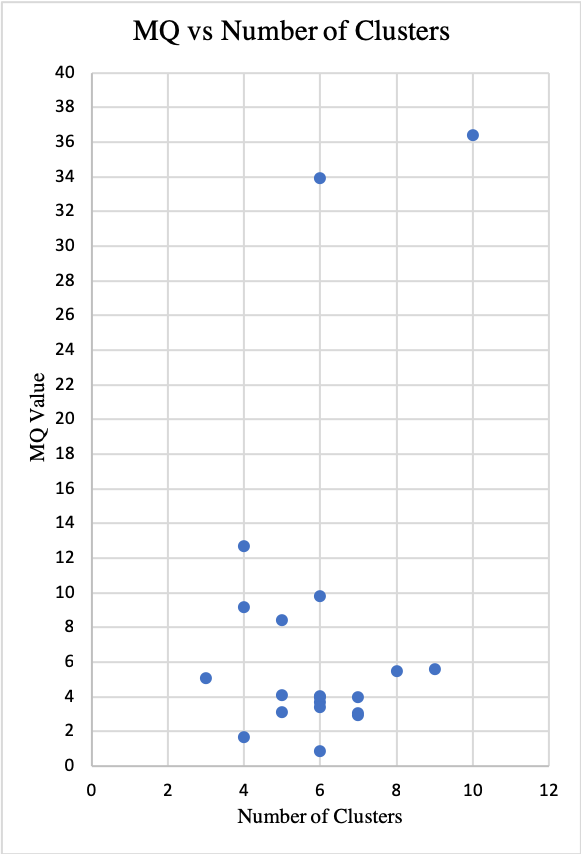
\includegraphics[width=0.8\columnwidth]{images/mq-vs-num-of-cluster-plot.png}
    \caption{\bn: A total of twenty times data against PartsUnlimitedMRP }
    \label{fig:mq-vs-num-of-cluster-plot}
\end{figure}

We excessively test the configuration of parameters of \bn and find that the extreme instability of the results come from the incremental MQ algorithm, which is used for optimizing the time complexity of calculating MQ values during iteration. Setting the algorithm to a naive approach significantly reduces the MQ value differences between runs. For a total of ten-time runs, \bn clustered the system into seven sub-components for nine times and eight sub-components for one time, and the MQ values for each run are within $[3.90, 3.95]$. We chose the run with MQ value equals to 3.95 as the final results for \bn.

In the PartsUnlimitedMRP benchmark, there exist duplicate classes when migrating from monolithic to microservice version. One main portion of such classes is exception classes. In an ideal decomposition, exception classes should be treated as "special classes" that belongs to an individual cluster, instead of grouping with other functional classes. Neither \bn nor \fs can distinguish the fundamental differences between these classes with other functional classes, and therefore, they group these exception classes with the domain that frequently uses these exceptions. 

\subsection{Threats to Validity}
\label{sec:threats}

% Selection of tools, selection of subjects, manual interpretation of the results.

Certain issues potentially undermine the validity of our results and our confidence in them. The three main aspects of issues come from the selection of tools, selection of subjects, and the non-uniqueness of the correct architecture.

First, we have only selected two extraction techniques among a variety of tools that could potentially be used as software system extraction techniques. Early work by Jonas Fritzsch, Justus Bogner, Alfred Zimmermann, and Stefan Wagner defined four categories for existing extraction techniques:
\begin{itemize}
    \item Static Code Analysis aided approaches
    \item Meta-Data aided approaches
    \item Workload-Data aided approaches
    \item Dynamic Microservice Composition approaches
\end{itemize}


\bn, which serves as one of the static code analysis aided approaches, uses the Module Dependency Graph extracted from source code as its input. \fs is one of the workload-data aided approaches, which focuses on using application operational data to determine a satisfactory decomposition. Our analysis does not cover the other two categories of techniques. We intentionally avoided choosing these two categories of techniques because these tools either require manually-intensive user input or do not have a result evaluation. This does not imply that these techniques cannot produce good results. Instead, it is hard to quantify all the human-involved efforts; therefore, these techniques are excluded from this comparative analysis.

Second, all three subjects of this analysis are relatively small, containing less than 50 modules, and this amplifies the differences in MoJoFM values of results and the ground-truths. To illustrate this, assume the case that exact one \textit{Move} operation is required to transform the extraction result to the ground-truth. For simplicity, we assume the maximum distance between two systems equal to the number of modules. Therefore, a system with ten modules  has  MoJoFM  value  =  90\%, while system with 100 modules has MoJoFM value = 99\%. These techniques likely produce such noises; therefore, these tools do not have a high similarity with the benchmarks. 

Besides, the three subjects use specific frameworks. For instance, PartsUnlimitedMRP is built on the Spring framework. This indicates that there exists dependencies from classes in the source code to the framework code and from the framework to the source code. Therefore, the dependencies of classes in the source code that are indirectly connected through the framework served as a "medium" are not considered. In other words, \bn may require additional framework-related inputs to generate more accurate results.

Third, for any software system, there is no single "correct" architecture. Even if the similarity of the result and the ground-truth is relatively low, it is still possible that the result suggests a reasonable architecture, which is much different from the ground-truth. Nevertheless, in terms of performance or any other aspect, it could potentially beat the ground-truth. Due to the consideration that the complexity level for all the subjects is relatively low, the possibility of having one architecture that completely different from the ground truth performs as good as the ground truth does is also low. 


